\chapter{Results}\label{c:r}
%
The code was found to scale linearly with integration step, number of Monte-Carlo repetitions (MC reps) and number of cores used---which are the best case scenarios; this is what everyone who does programming hopes for. There were some minor variations from exact linearity but their randomness is due to the model's Monte-Carlo characteristics. It was also found that accuracy is more dependent on the number of MC reps than the size of the integration step, $ h $. In fact, the integration step could be made relatively large (how large depends on the problem) without significantly affecting accuracy, but drastically reducing execution time. There was also no significant difference between using $ \gamma = \dfrac{\sqrt{3}-1}{2} $ and $ \gamma = 0.366 $ \cite{project}---the actual value is very similar, but there is no need to evaluate square roots and divisions all the time if we use the numerical approximation; \cite{project} gives the theoretical justification for this value, but it can be adjusted on a case by case basis. Accuracy was also not noticeably affected by parallel runs, presumably due to the random number generator used---which is thread safe---but not optimal for parallelisation, because it generates numbers in sequence from a single source rather than in parallel\footnote{See \url{https://gcc.gnu.org/onlinedocs/gfortran/RANDOM_005fNUMBER.html}} (this only affects execution speed).

The number of MC reps $ = 15000 $ and the value of $ \gamma = 0.366 $ unless stated otherwise. Reflections are denoted as $ R $ and transmissions as $ T $, electronic transitions from an initial state, $ i $, to a final state, $ f $, are denoted as $ f \leftarrow i $. 

All calculations were carried out on a computer equipped with an Intel i7-3770k processor overclocked to 4.3 GHz, $ 2\times4 $ Gb Kingston RAM overclocked to 1660 MHz, mounted on a Gigabyte GA-Z77X-UD3H motherboard (the video card is irrelevant because all calculations were processor bound), all functioning on the {\ubuntumono ubuntu 14.04 LTS} operating system. The code was compiled with the \texttt{gfortran} module from the \texttt{GNU} compiler collection \texttt{gcc 4.9.2} \footnote{See \url{https://gcc.gnu.org/}}.
%
\section{Single Avoided Crossing}
%
Being the simplest system, the single avoided crossing problem was used to test code's robustness. \Crefrange{f:scc}{f:sc1t} show results for $ i = 1 $ while \crefrange{f:sci2}{f:sc2t} show the results for $ i = 2 $. Despite this being the simplest problem tackled herein, it presents some fairly interesting behaviours. The results for when $ i = 1 $ are very similar---though not exactly the same---as those found in \cite{project}. However, this is most likely down to the fact that they used $ 50000\text{--}100000$ trajectories as well as there being a strong possibility that the compiler, RNG, and integration step differ.

\Cref{f:scc} shows a comparison between two different integration step sizes, there is no significant difference in accuracy between them both.
\begin{figure}
\centering
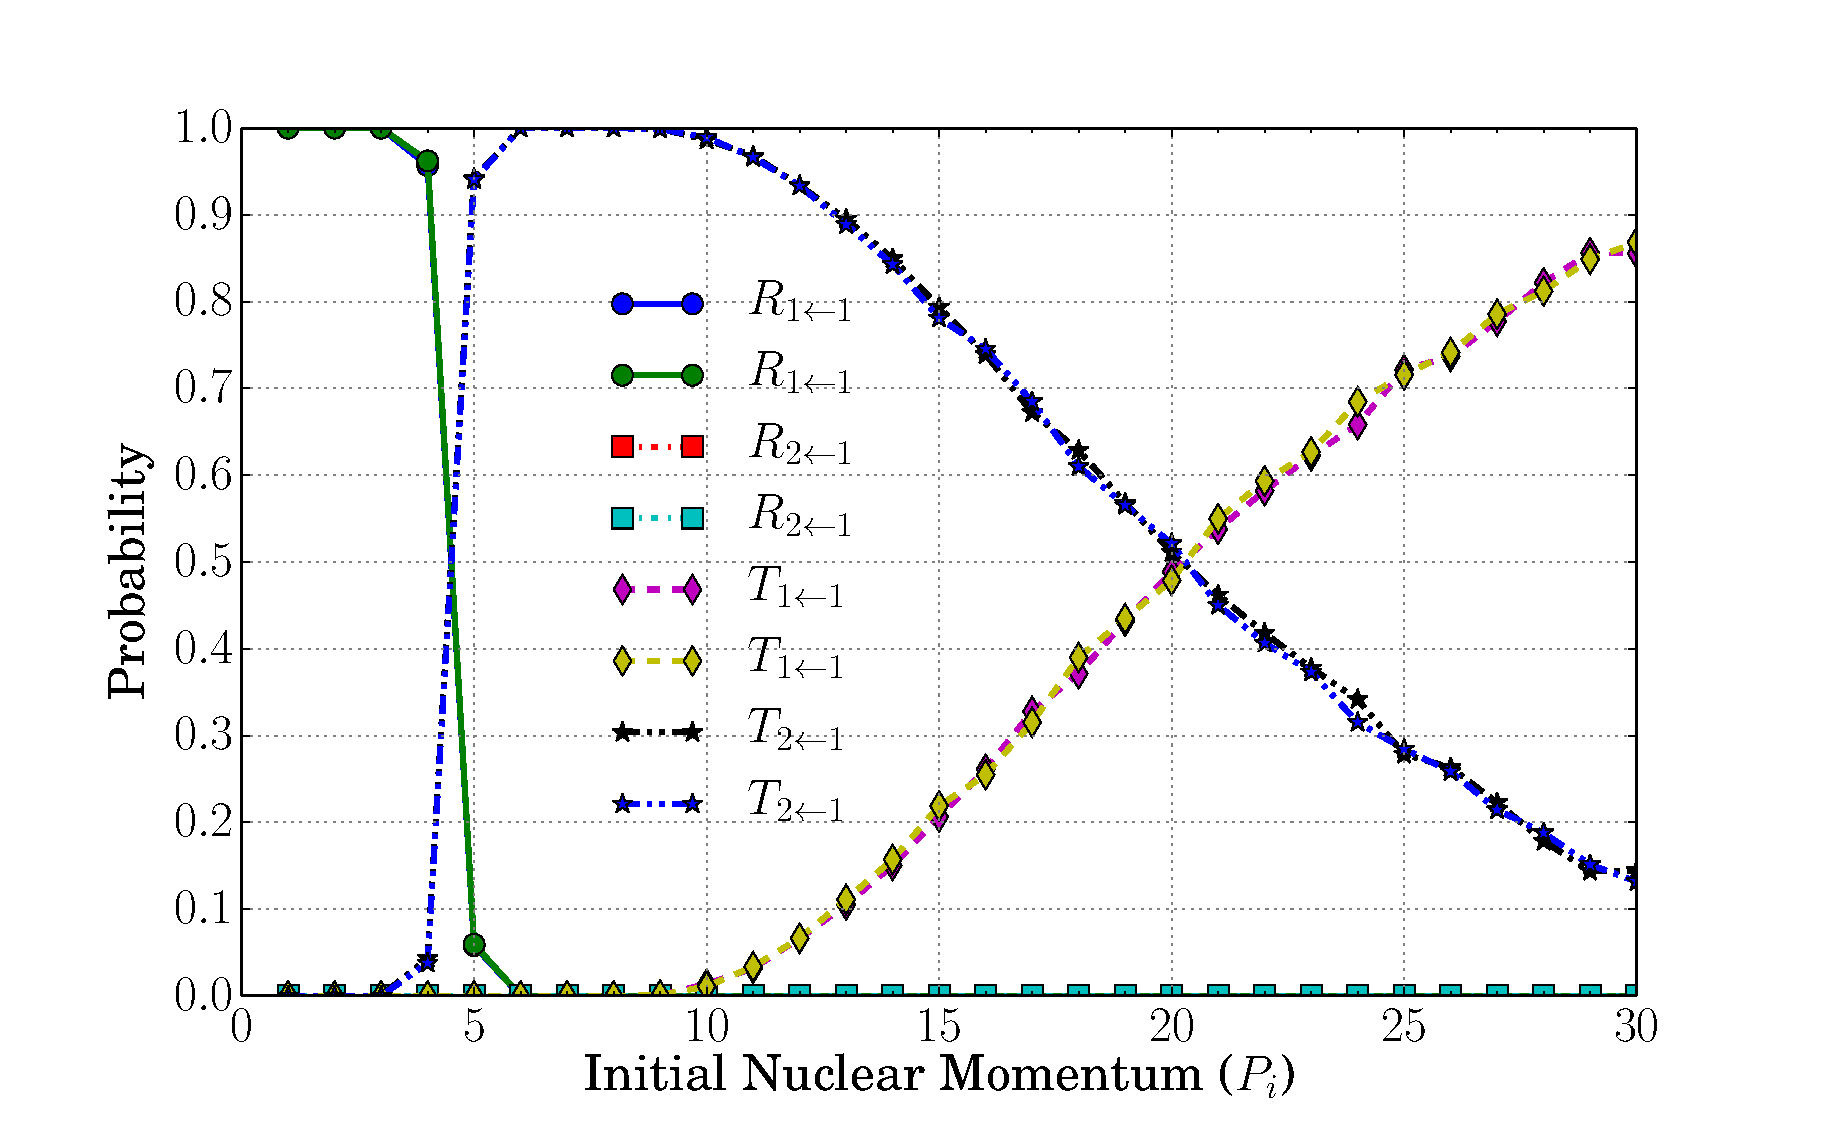
\includegraphics[scale=0.5]{sc_prob_1oip_vs_1o5ip.eps}
\caption[Single avoided crossing: comparison between integration step size. $ i = 1 $.]{Comparison between $ h = (5P_{i})^{-1} $ (appearing first in the legend) and $ h = P_{i}^{-1} $. $ \gamma = \frac{\sqrt{3} - 1}{2}$ in both cases. $ i = 1 $.}
\label{f:scc}
\end{figure}
\Cref{f:sclh} shows the results for very large values of $ h $, there is no significant difference between using large or small values of $ h $.
\begin{figure}
\centering
\includegraphics[scale=0.5]{sc_prob_lh.eps}
\caption[Single avoided crossing: large integration step. $ i = 1 $.]{Transition probabilities for $ R $ and $ T $, $ h = (0.012P_{i})^{-1} $. $ i = 1 $. Computational time $ = 8$ min. $ 7.35 $ s.}
\label{f:sclh}
\end{figure}
\Cref{f:scpar} shows a two-core parallel run, there is no significant difference in accuracy compared to single-core calculations.
\begin{figure}
\centering
\includegraphics[scale=0.5]{sc_prob_parallel.eps}
\caption[Single avoided crossing: parallel calculations. $ i = 1 $.]{Parallel calculations on two cores (7500 MC reps per core), $ h = (5P_{i})^{-1} $. No significant deviation from single-core calculations. $ i = 1 $.}
\label{f:scpar}
\end{figure}

First, we shall tackle the case where $ i = 1 $. The behaviour of \roo, whose probability is seen to rapidly decline as nuclear momentum increases, can be explained by referring back to \cref{f:pessc}. For small values of nuclear momentum, there is not enough kinetic energy to scale over the potential barrier (akin to an `activation energy') and continue in the original direction, thus the particle is reflected back, preventing its electronic states from interacting, as seen in \cref{sf:scr11,sf:scr11e}. \rto~is similarly explained; once there is enough kinetic energy to reach a point where a transition is likely to happen, there would also be enough energy to continue on to the other side. Thus \rto~remains relatively close to zero throughout. The others can be explained by the fact that transition probabilities are not only a function of the distance between adiabatic PES, but also of the time it takes the particle to move away from regions where electronic coupling is strong. This explains the behaviour of \tto~and \too. For \tto~lower nuclear momenta allow more time for an electronic transition to occur as seen in \cref{sf:sct21,sf:sct21e}; however, after a certain value of nuclear momentum, it begins to decrease in favour of \too~because the particle travels so fast, it cannot interact long enough to undergo an electronic transition, as shown in \cref{sf:sct11,sf:sct21e}.

\begin{figure}
\begin{subfigure}[t]{0.5\textwidth}
\centering
\includegraphics[width=\textwidth]{sc_traj_r11.eps}
\caption[Single avoided crossing: \roo~trajectory.]{\roo~trajectory.}
\label{sf:scr11}
\end{subfigure}
~
\begin{subfigure}[t]{0.5\textwidth}
\centering
\includegraphics[width=\textwidth]{sc_traj_r11_e.eps}
\caption[Single avoided crossing: \roo~trajectory, zoom into $ n_{1}~\text{and}~n_{2} $.]{\roo~trajectory, zoom into $ n_{1}~\text{and}~n_{2} $.}
\label{sf:scr11e}
\end{subfigure}

\begin{subfigure}[t]{0.5\textwidth}
\centering
\includegraphics[width=\textwidth]{sc_traj_t21.eps}
\caption[Single avoided crossing: \tto~trajectory.]{\tto~trajectory.}
\label{sf:sct21}
\end{subfigure}
~
\begin{subfigure}[t]{0.5\textwidth}
\centering
\includegraphics[width=\textwidth]{sc_traj_t21_e.eps}
\caption[Single avoided crossing: \tto~trajectory, zoom into $ n_{1}~\text{and}~n_{2} $.]{\tto~trajectory, zoom into $ n_{1}~\text{and}~n_{2} $.}
\label{sf:sct21e}
\end{subfigure}

\begin{subfigure}[t]{0.5\textwidth}
\centering
\includegraphics[width=\textwidth]{sc_traj_t11.eps}
\caption[Single avoided crossing: \too~trajectory.]{\too~trajectory.}
\label{sf:sct11}
\end{subfigure}
~
\begin{subfigure}[t]{0.5\textwidth}
\centering
\includegraphics[width=\textwidth]{sc_traj_t11_e.eps}
\caption[Single avoided crossing: \too~trajectory, zoom into $ n_{1}~\text{and}~n_{2} $.]{\too~trajectory, zoom into $ n_{1}~\text{and}~n_{2} $.}
\label{sf:sct11e}
\end{subfigure}
\caption[Single avoided crossing: trajectory examples. $ i = 1 $.]{Trajectory examples.  $ i = 1 $.}
\label{f:sc1t}
\end{figure}

\begin{figure}
\centering
\includegraphics[scale=0.5]{sc_prob_i2.eps}
\caption[Single avoided crossing. $ i = 2 $]{Transition probabilities for $ R $ and $ T $, $ h = (0.012P_{i})^{-1} $. $ i = 2 $. Computational time $ = 7$ min. $ 47.74 $ s.}
\label{f:sci2}
\end{figure}
In the case of $ i = 2 $ only one graph is provided (\cref{f:sci2}), as tests yielded similar results as previously demonstrated. In this case, the system's behaviour is more nuanced, but is explained by the same reasons. The \rot~transition remains effectively zero throughout, because at such low nuclear momenta two things can happen: the particle can be reflected back along $ H_{22} $ by the off-diagonal PES---corresponding to the \rtt~transition, as seen in \cref{sf:scr22,sf:scr22e} (in fact the particle keeps getting bounced back time and time again until it finally leaves the integration area as a reflection)---or it moves down to the lower energy state, where the surplus potential energy is converted into kinetic energy (conservation of energy) and a \tot~transition is observed, as seen in \cref{sf:sct12,sf:sct12e}. For higher values of nuclear momentum, the particle has enough energy to be transmitted, but there is not enough time for the particle's electronic states to interact, and a \ttt~is observed instead, shown in \cref{sf:sct22,sf:sct22e}. The higher the nuclear momentum the less time there is and the likelier this transition becomes.

\begin{figure}
\begin{subfigure}[t]{0.5\textwidth}
\centering
\includegraphics[width=\textwidth]{sc_traj_r22.eps}
\caption[Single avoided crossing: \rtt~trajectory.]{\rtt~trajectory.}
\label{sf:scr22}
\end{subfigure}
~
\begin{subfigure}[t]{0.5\textwidth}
\centering
\includegraphics[width=\textwidth]{sc_traj_r22_e.eps}
\caption[Single avoided crossing: \rtt~trajectory, zoom into $ n_{1}~\text{and}~n_{2} $.]{\rtt~trajectory, zoom into $ n_{1}~\text{and}~n_{2} $.}
\label{sf:scr22e}
\end{subfigure}

\begin{subfigure}[t]{0.5\textwidth}
\centering
\includegraphics[width=\textwidth]{sc_traj_t12.eps}
\caption[Single avoided crossing: \tot~trajectory.]{\tot~trajectory.}
\label{sf:sct12}
\end{subfigure}
~
\begin{subfigure}[t]{0.5\textwidth}
\centering
\includegraphics[width=\textwidth]{sc_traj_t12_e.eps}
\caption[Single avoided crossing: \tot~trajectory, zoom into $ n_{1}~\text{and}~n_{2} $.]{\tot~trajectory, zoom into $ n_{1}~\text{and}~n_{2} $.}
\label{sf:sct12e}
\end{subfigure}

\begin{subfigure}[t]{0.5\textwidth}
\centering
\includegraphics[width=\textwidth]{sc_traj_t22.eps}
\caption[Single avoided crossing: \ttt~trajectory.]{\ttt~trajectory.}
\label{sf:sct22}
\end{subfigure}
~
\begin{subfigure}[t]{0.5\textwidth}
\centering
\includegraphics[width=\textwidth]{sc_traj_t22_e.eps}
\caption[Single avoided crossing: \ttt~trajectory, zoom into $ n_{1}~\text{and}~n_{2} $.]{\ttt~trajectory, zoom into $ n_{1}~\text{and}~n_{2} $.}
\label{sf:sct22e}
\end{subfigure}
\caption[Single avoided crossing: trajectory examples. $ i = 2 $.]{Trajectory examples. $ i = 2 $.}
\label{f:sc2t}
\end{figure}
%
\section{Double Avoided Crossing}\label{s:rdac}
%
\Crefrange{f:dc1}{f:dc1t} show results for $ i = 1 $ while \crefrange{f:dc2}{f:dc2t} show the results for $ i = 2 $. Again the results for when $ i = 1 $ are very similar---but not exactly the same---as those found in \cite{project}. Which can be attributed to the same factors as before. In our case $ E_{i} $ is the mean total initial energy, which could also contribute to the differences with published results.

\Cref{f:dc1} shows the results for small values of $ h $, while \cref{f:dclh} uses large values of $ h $. There is no significant difference between the two.
\begin{figure}
\centering
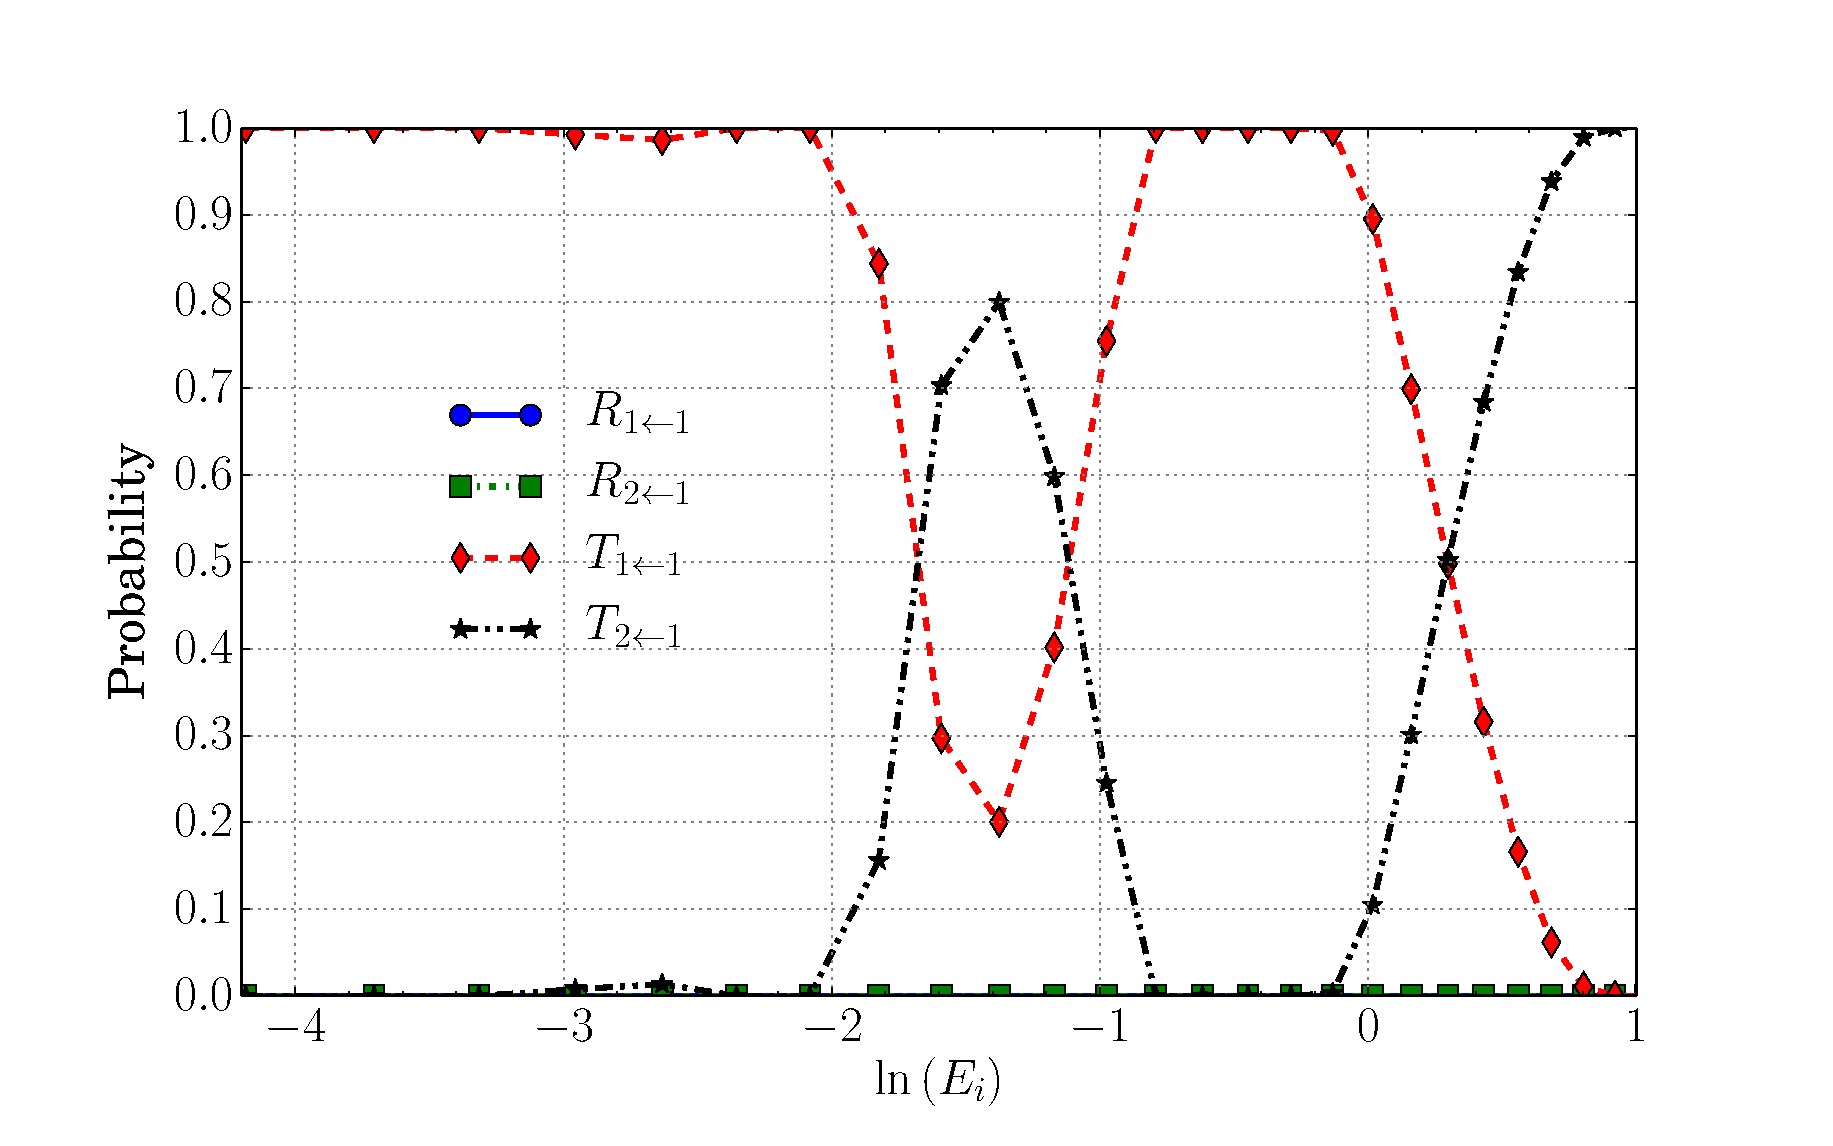
\includegraphics[scale=0.5]{dc_prob_1o5ip.eps}
\caption[Double avoided crossing: small integration step. $ i = 1 $.]{Transition probabilities for $ R $ and $ T $, $ h =(5 P_{i})^{-1} $. $ i = 1 $.}
\label{f:dc1}
\end{figure}
\begin{figure}
\centering
\includegraphics[scale=0.5]{dc_prob_lh.eps}
\caption[Double avoided crossing: large integration step. $ i = 1 $.]{Transition probabilities for $ R $ and $ T $ for $ h = (0.0125P_{i})^{-1} $. $ i = 1 $. Computational time $ = 7$ min. $ 33.29 $ s.}
\label{f:dclh}
\end{figure}
\Cref{f:dcpar} shows a two-core parallel run. There is no significant difference between this and \cref{f:dc1}.
\begin{figure}
\centering
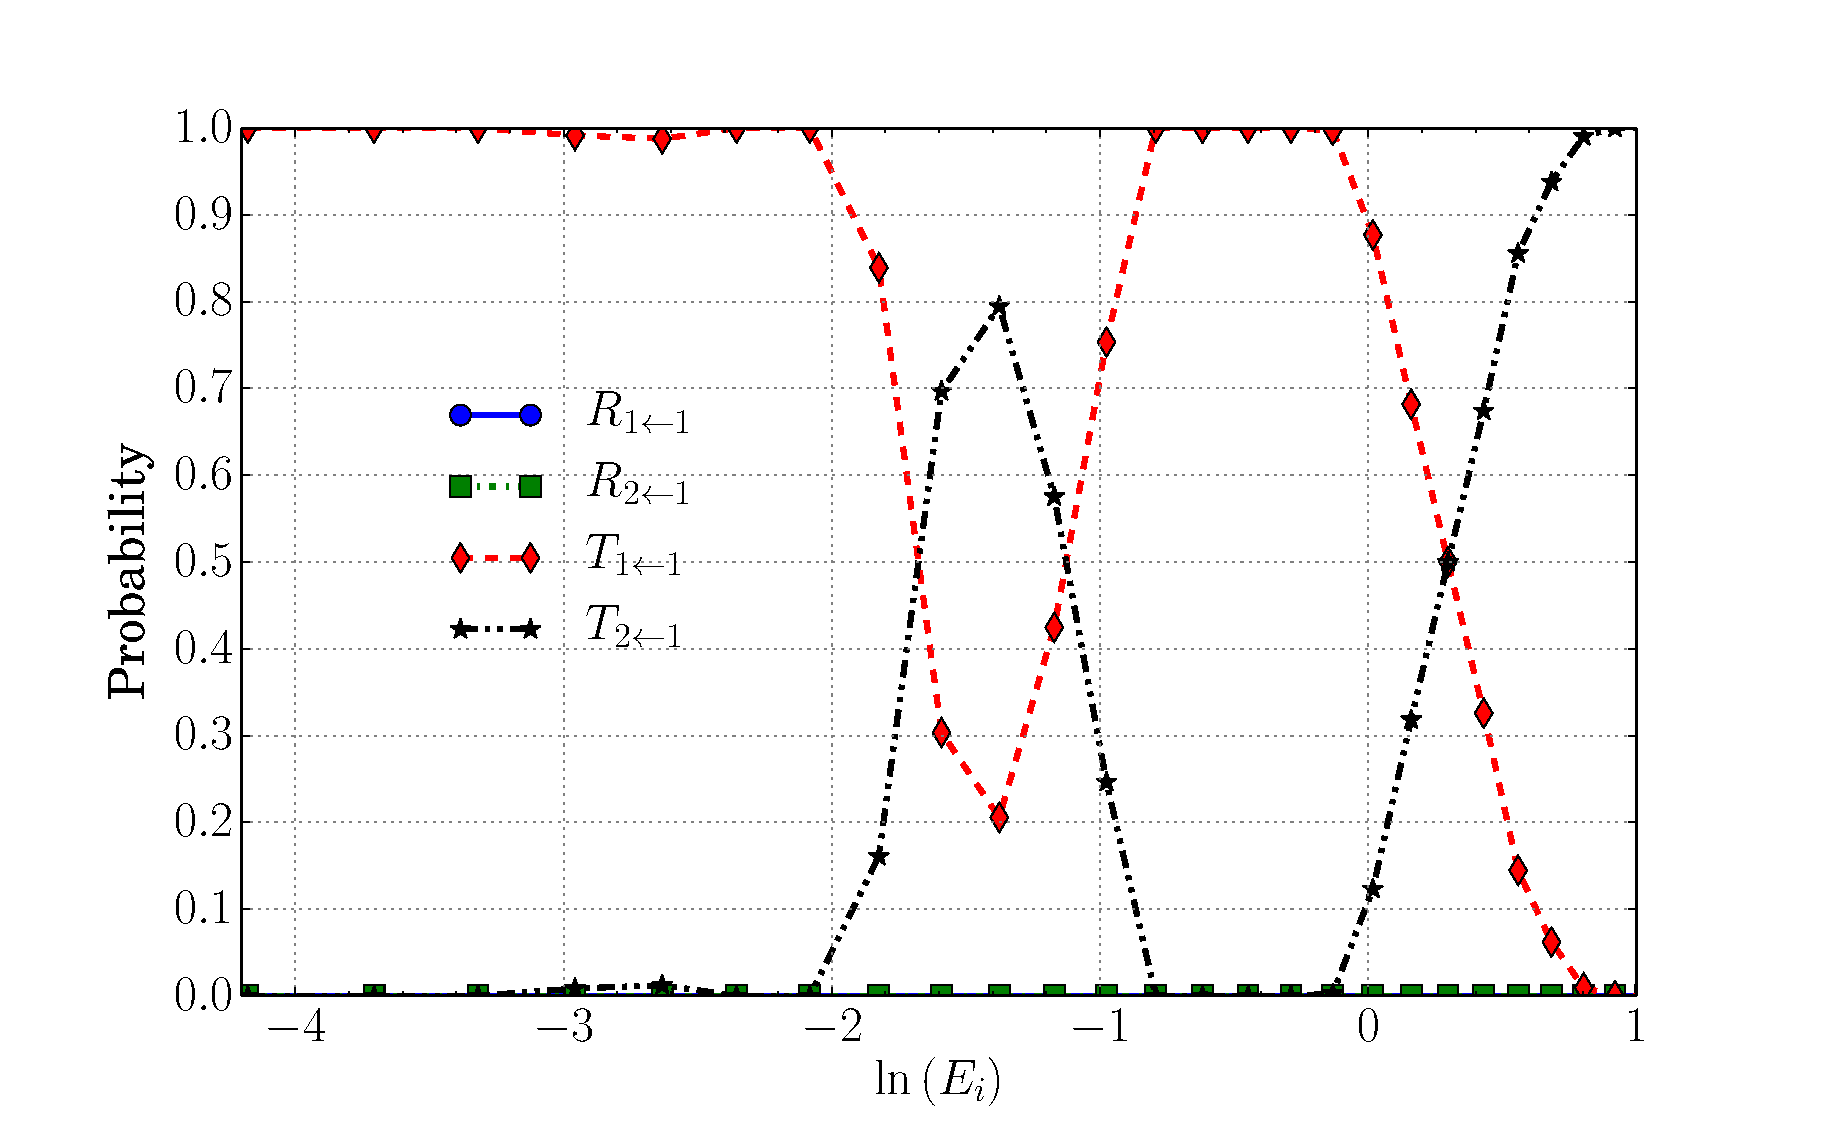
\includegraphics[scale=0.5]{dc_prob_parallel.eps}
\caption[Double avoided crossing: parallel calculations. $ i = 1 $.]{Parallel calculations on two cores (7500 MC reps per core), $ h = (5P_{i})^{-1} $. No significant deviation from single-core calculations. $ i = 1 $.}
\label{f:dcpar}
\end{figure}

Once more, we shall first analyse the behaviour for $ i = 1 $, shown in \crefrange{f:dc1}{f:dcpar}. The lack of \roo~and \rto~transitions is easily explained by the fact there is no energy barrier in either the diagonal diabatic or adiabatic PES as seen in \cref{f:pesdc,f:apesdc}. Therefore the particle only requires a small amount of momentum for the it to be transmitted. In fact, in low momentum tests (\cref{sf:lm,sf:lme}), the particle was accelerated by the adiabatic energy wells (potential energy was transferred into kinetic energy). The other interesting feature is the presence the Stückelberg oscillations for both \too~and \tto, which are often attributed to quantum interference effects clearly seen in \cref{sf:t11e,sf:t21e}. In order to comprehend these one must only turn to \cref{f:delapesdc}, which shows the difference between adiabatic PES. One can see that $ E_{2} - E_{1} $ varies quickly and by relatively large amounts. For small momenta, the particle generally does not have enough energy to switch electronic states, leading to the relatively flat appearance of both \too~and \tto~from $ -4~\text{to}~-2 $. However, as momentum increases, there is enough energy to make one jump but not a lot to make the second one, leading to the behaviour seen from $ -2~\text{to}~-1 $. As momentum keeps increasing, there is enough energy for the second jump, and we get the behaviour we see from $ -1~\text{to}~0 $. Finally, when momentum is very large, the particle carries out one jump and does not linger long enough around the second minimum energy difference range, leading to the behaviour we see from $ 0~\text{to}~1 $. \Cref{f:dc1t} contains trajectory examples which support these allegations.

\begin{figure}
\begin{subfigure}[t]{0.5\textwidth}
\centering
\includegraphics[width=\textwidth]{dc_traj_t11.eps}
\caption[Double avoided crossing: \too~trajectory.]{\too~trajectory.}
\label{sf:t11}
\end{subfigure}
~
\begin{subfigure}[t]{0.5\textwidth}
\centering
\includegraphics[width=\textwidth]{dc_traj_t11_e.eps}
\caption[Double avoided crossing: \too~trajectory, zoom into $ n_{1}~\text{and}~n_{2} $.]{\too~trajectory, zoom into $ n_{1}~\text{and}~n_{2} $.}
\label{sf:t11e}
\end{subfigure}

\begin{subfigure}[t]{0.5\textwidth}
\centering
\includegraphics[width=\textwidth]{dc_traj_t21.eps}
\caption[Double avoided crossing: \tto~trajectory.]{\tto~trajectory.}
\label{sf:t21}
\end{subfigure}
~
\begin{subfigure}[t]{0.5\textwidth}
\centering
\includegraphics[width=\textwidth]{dc_traj_t21_e.eps}
\caption[Double avoided crossing: \tto~trajectory, zoom into $ n_{1}~\text{and}~n_{2} $.]{\tto~trajectory, zoom into $ n_{1}~\text{and}~n_{2} $.}
\label{sf:t21e}
\end{subfigure}

\begin{subfigure}[t]{0.5\textwidth}
\centering
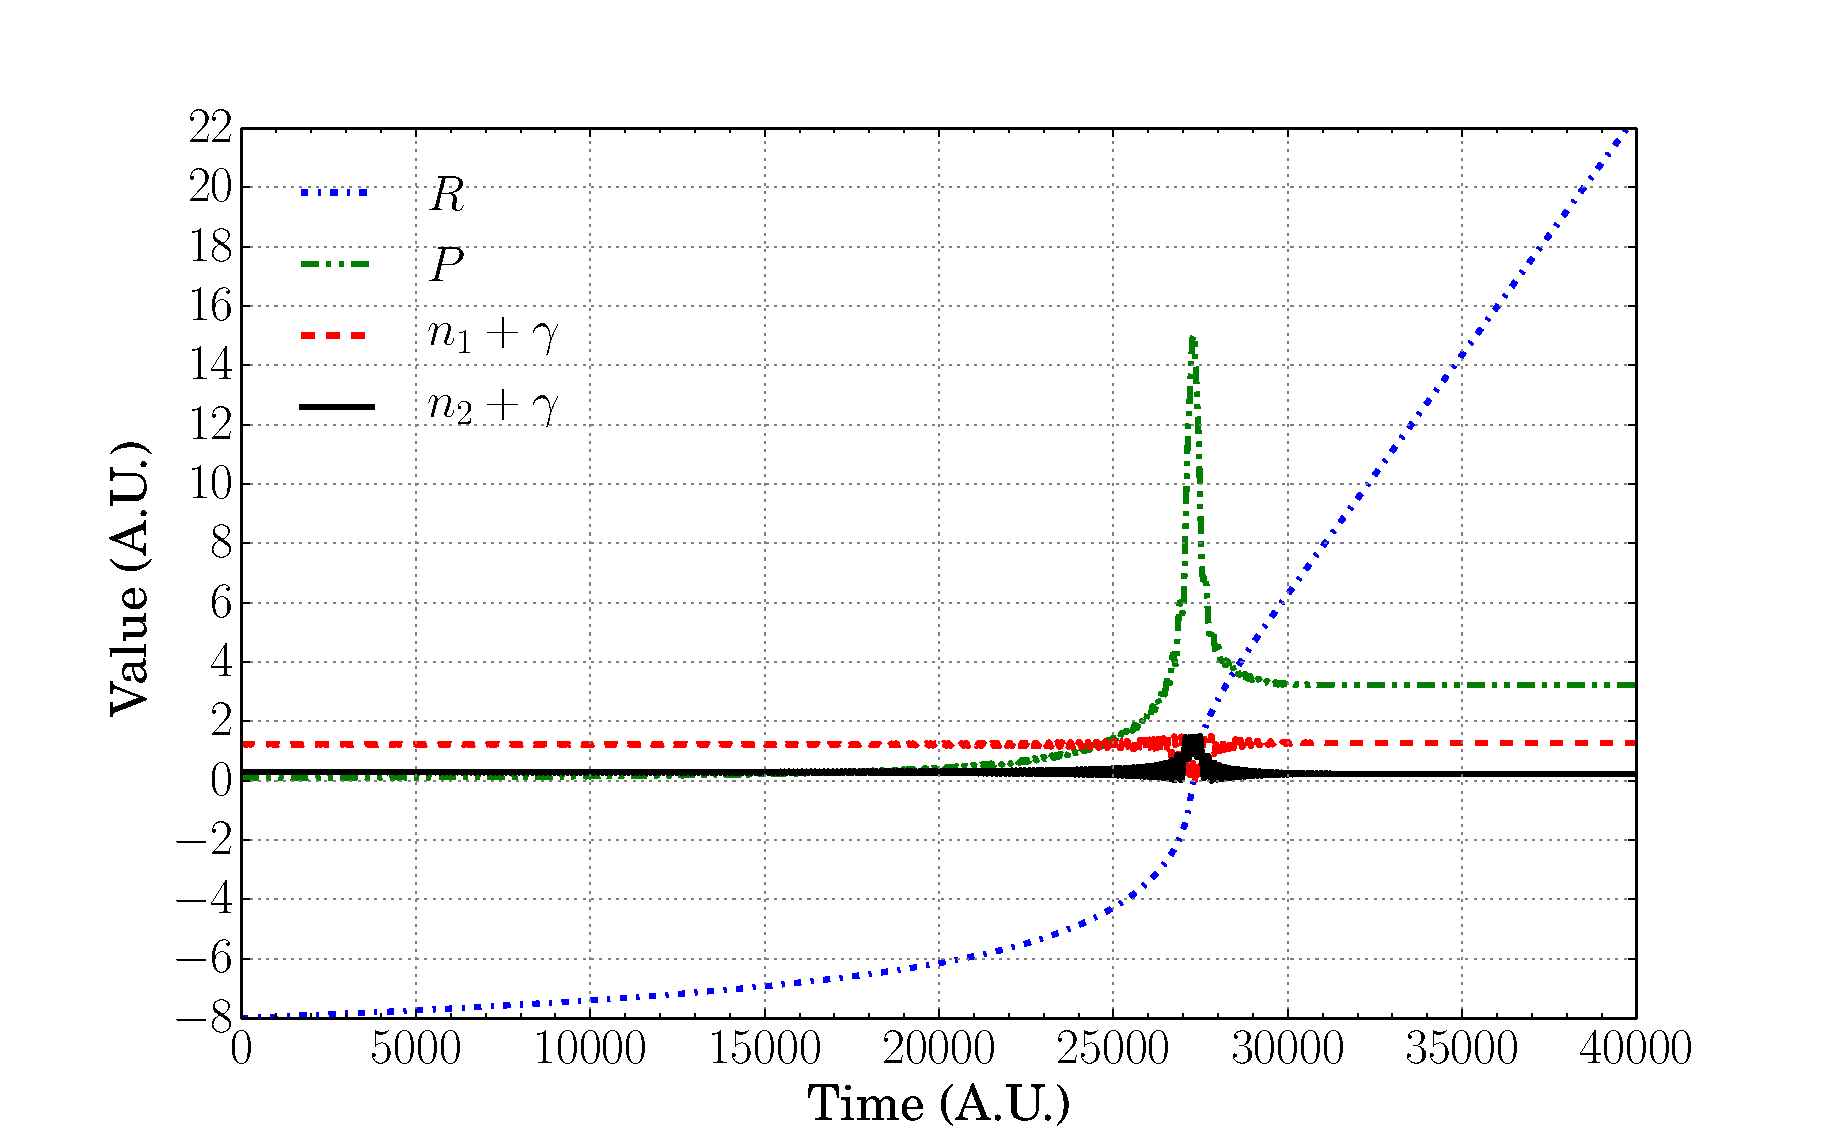
\includegraphics[width=\textwidth]{dc_traj_low_momentum.eps}
\caption[Double avoided crossing: low nuclear momentum trajectory.]{Low nuclear momentum trajectory.}
\label{sf:lm}
\end{subfigure}
~
\begin{subfigure}[t]{0.5\textwidth}
\centering
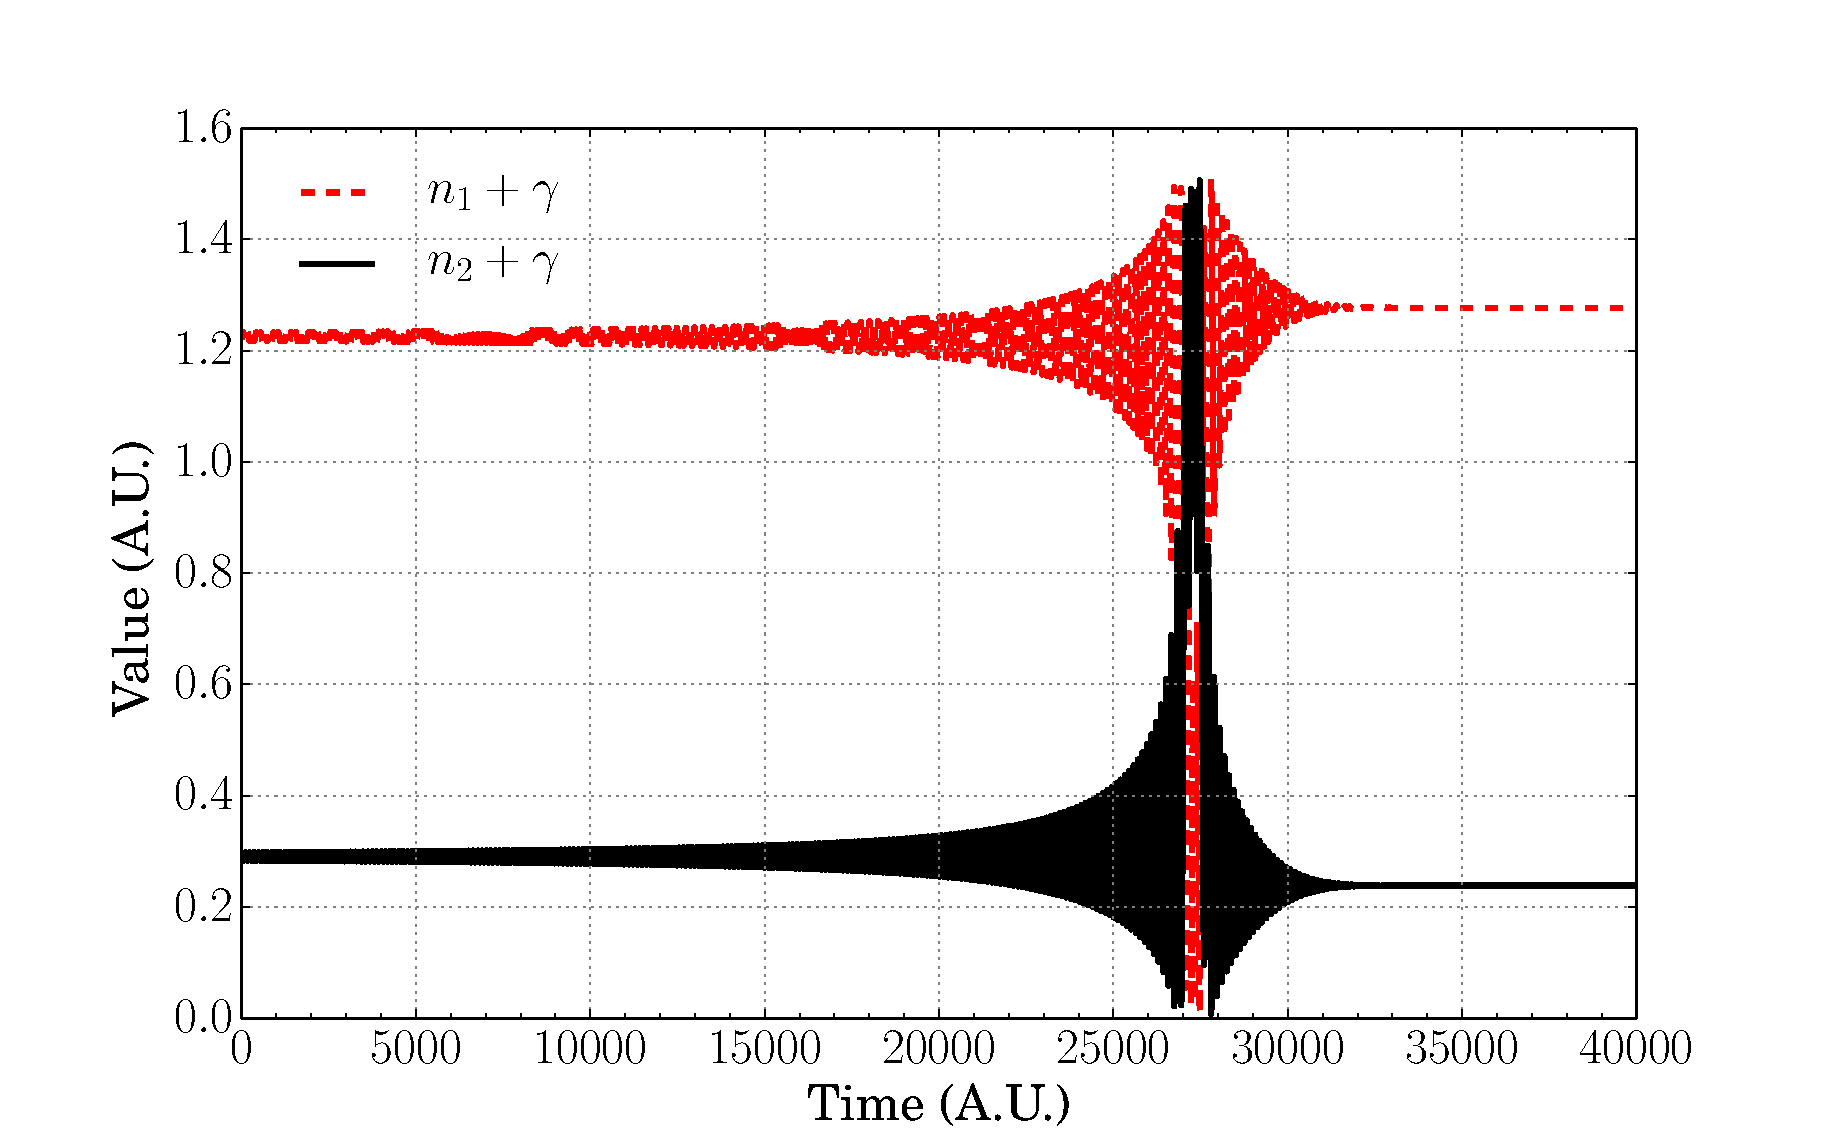
\includegraphics[width=\textwidth]{dc_traj_low_momentum_e.eps}
\caption[Double avoided crossing: low nuclear momentum trajectory, zoom into $ n_{1}~\text{and}~n_{2} $.]{Low nuclear momentum trajectory, zoom into $ n_{1}~\text{and}~n_{2} $.}
\label{sf:lme}
\end{subfigure}
\caption[Double avoided crossing: trajectory examples. $ i = 1 $.]{Trajectory examples. $ i = 1 $.}
\label{f:dc1t}
\end{figure}

\begin{figure}
\centering
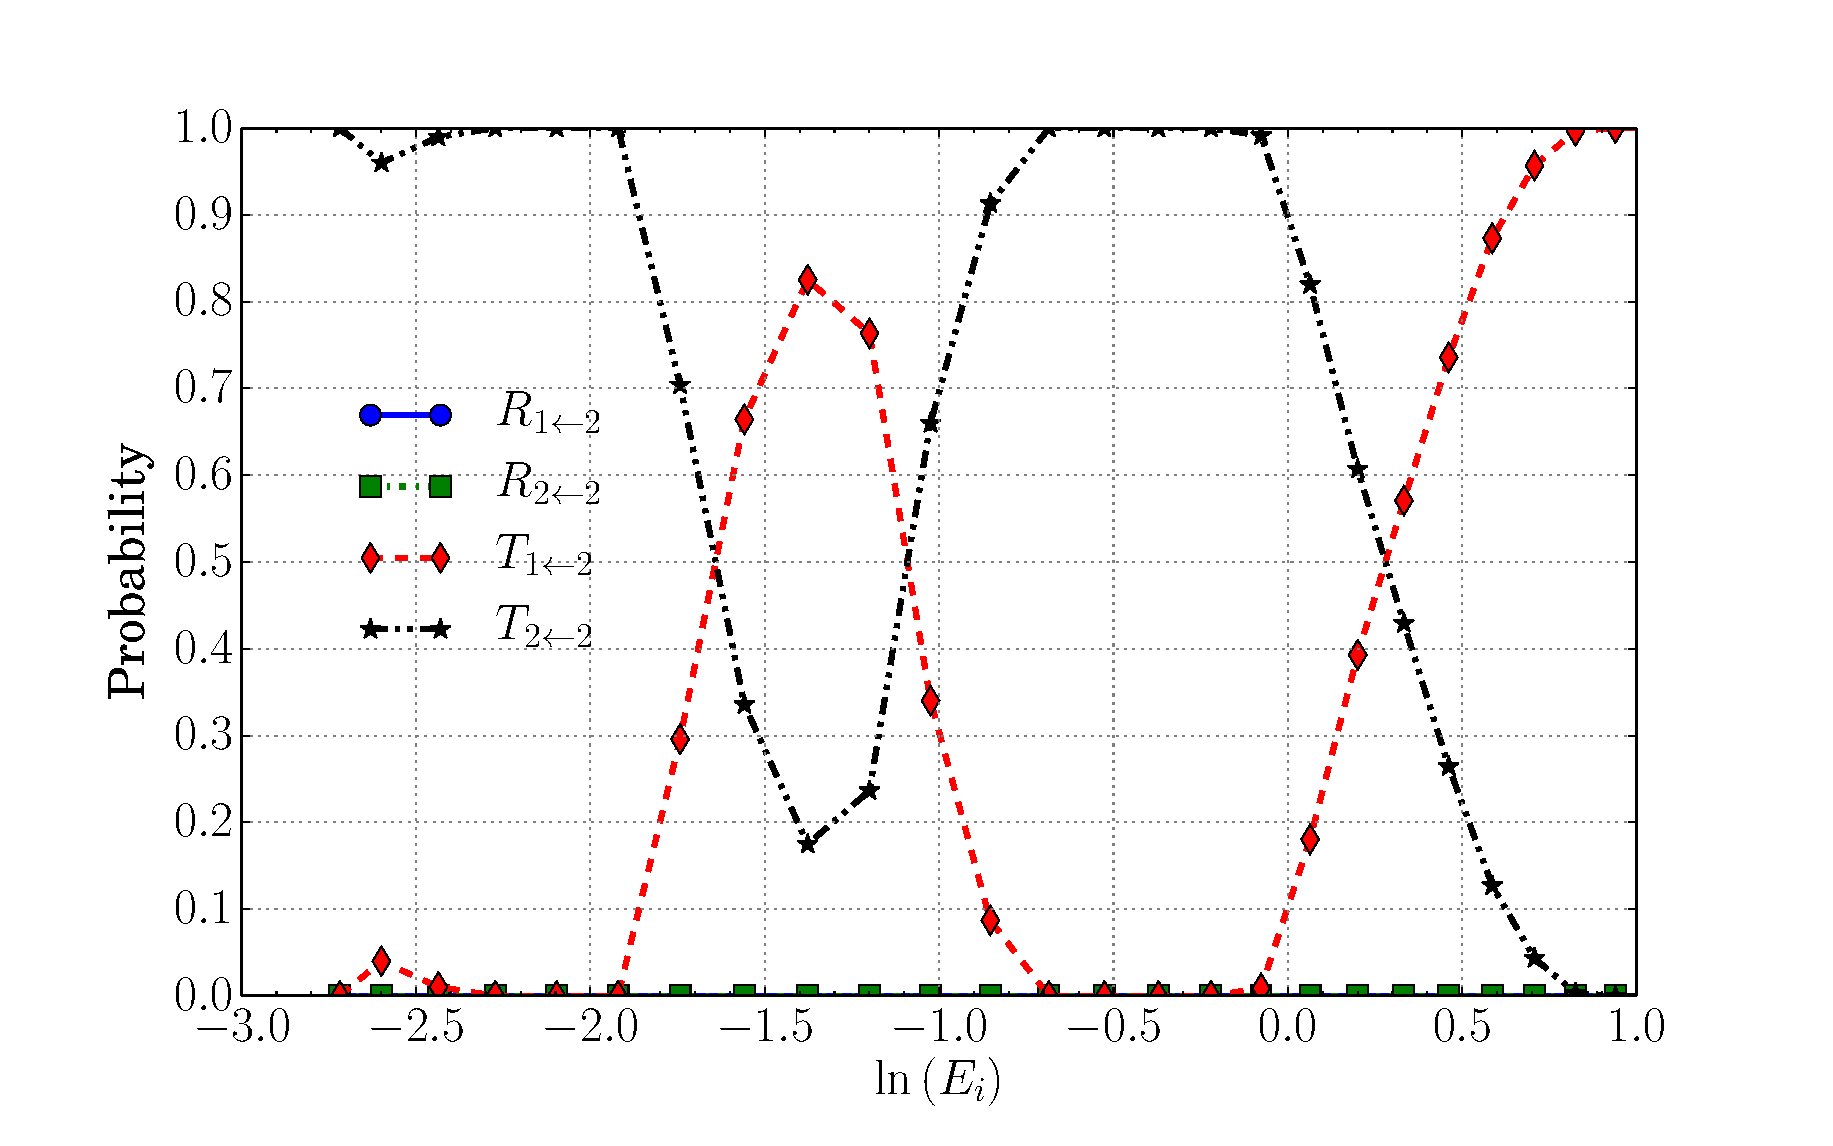
\includegraphics[scale=0.5]{dc_prob_i2.eps}
\caption[Double avoided crossing. $ i = 2 $]{Transition probabilities for $ R $ and$ T $ for $ h = (0.0125P_{i})^{-1} $. $ i = 2 $. Computational time $ = 10$ min. $ 41.63 $ s.}
\label{f:dc2}
\end{figure}
When the $ i = 2 $ as is the case in \cref{f:dc2}, the behaviour is very similar but inverted with respect to $ i = 1 $. In other words, the transmission which preserves the initial state, \ttt~in \cref{f:dc2}, is very similar in shape to the transmission which preserves the initial state, \too~in \cref{f:dc1}. And the transmission which does not preserve the initial state, \tot~in \cref{f:dc2}, is also very qualitatively similar to the transition which does not preserve the initial state, \tto~in \cref{f:dc1}. Which means they have similar explanations; the only variation being the precise points at which these `domains' appear. Trajectory examples are provided in \cref{f:dc2t}.

\begin{figure}
\begin{subfigure}[t]{0.5\textwidth}
\centering
\includegraphics[width=\textwidth]{dc_traj_t12.eps}
\caption[Double avoided crossing: \tot~trajectory.]{\tot~trajectory.}
\end{subfigure}
~
\begin{subfigure}[t]{0.5\textwidth}
\centering
\includegraphics[width=\textwidth]{dc_traj_t12_e.eps}
\caption[Double avoided crossing: \tot~trajectory, zoom into $ n_{1}~\text{and}~n_{2} $.]{\tot~trajectory, zoom into $ n_{1}~\text{and}~n_{2} $.}
\end{subfigure}

\begin{subfigure}[t]{0.5\textwidth}
\centering
\includegraphics[width=\textwidth]{dc_traj_t22.eps}
\caption[Double avoided crossing: \ttt~trajectory.]{\ttt~trajectory.}
\end{subfigure}
~
\begin{subfigure}[t]{0.5\textwidth}
\centering
\includegraphics[width=\textwidth]{dc_traj_t22_e.eps}
\caption[Double avoided crossing: \ttt~trajectory, zoom into $ n_{1}~\text{and}~n_{2} $.]{\ttt~trajectory, zoom into $ n_{1}~\text{and}~n_{2} $.}
\end{subfigure}

\begin{subfigure}[t]{0.5\textwidth}
\centering
\includegraphics[width=\textwidth]{dc_traj_low_momentum_2.eps}
\caption[Double avoided crossing: low nuclear momentum trajectory.]{Low nuclear momentum trajectory.}
\end{subfigure}
~
\begin{subfigure}[t]{0.5\textwidth}
\centering
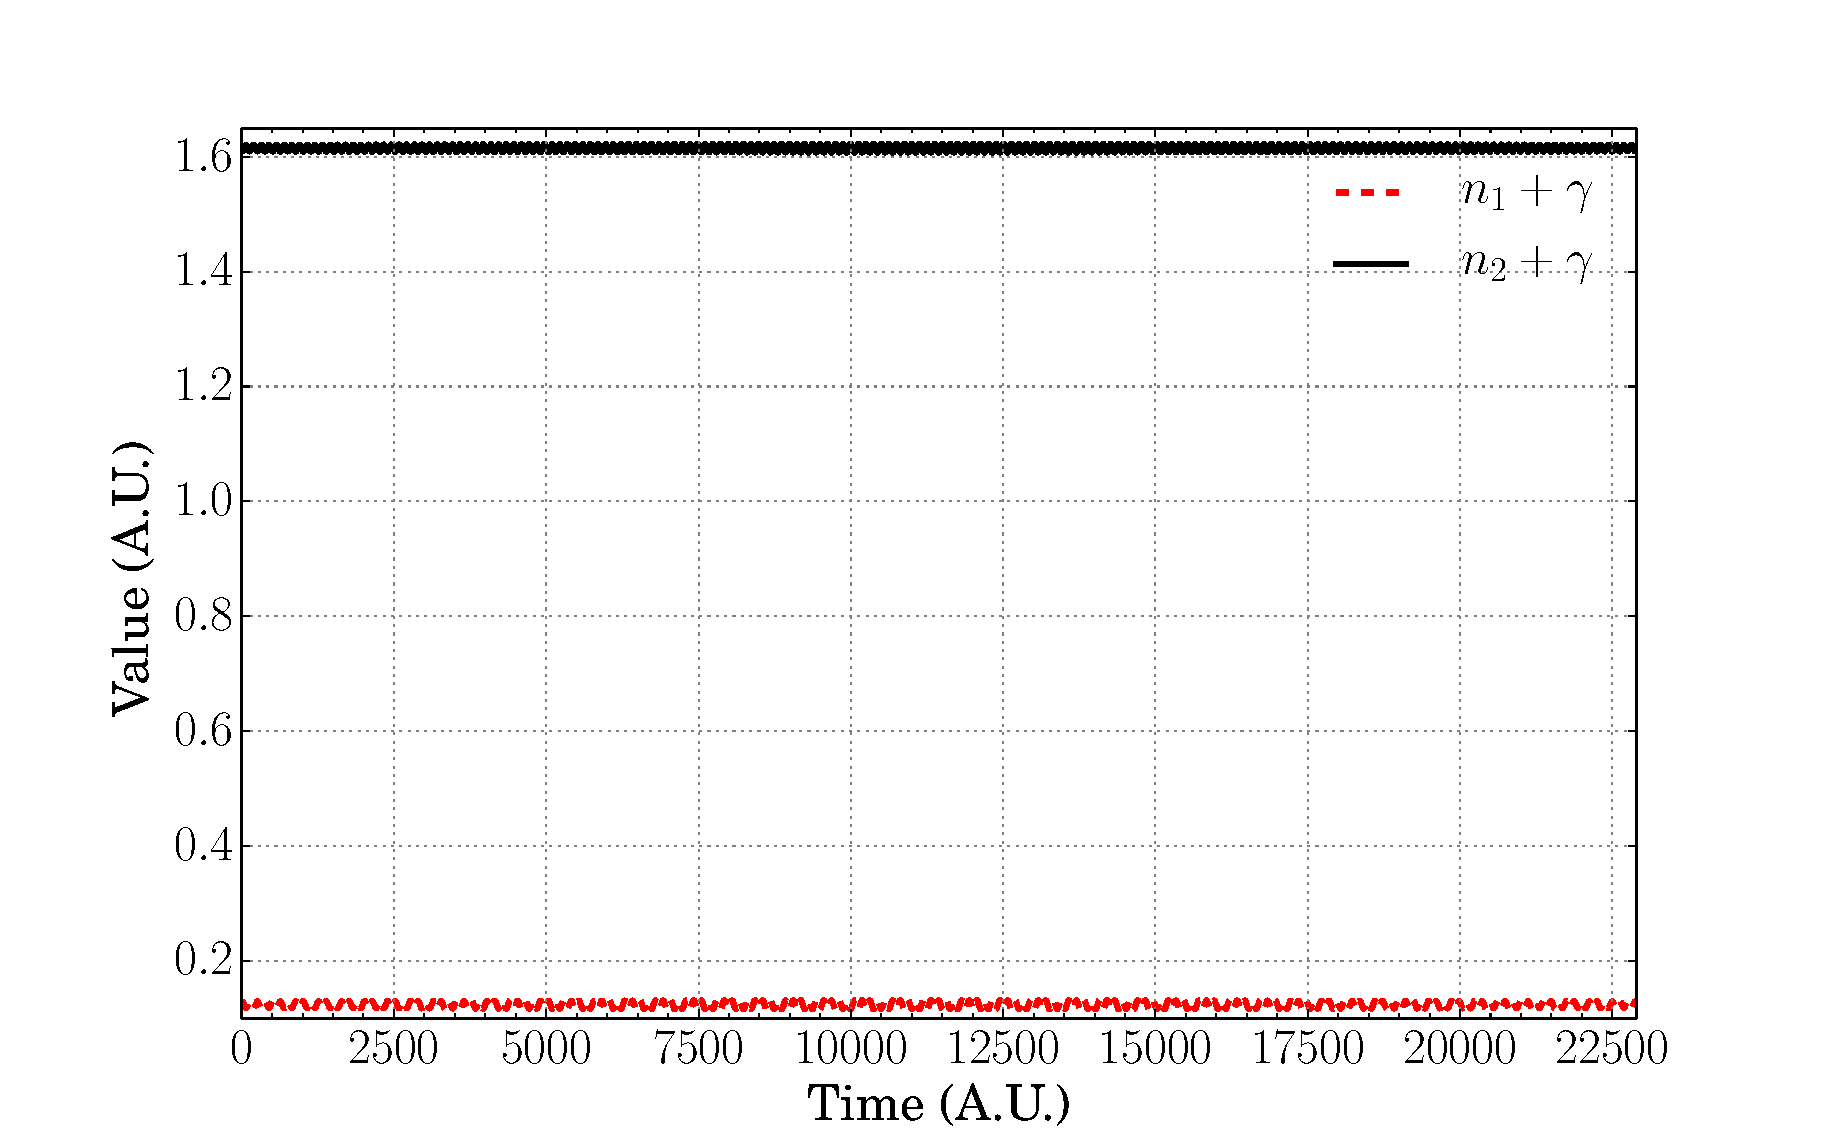
\includegraphics[width=\textwidth]{dc_traj_low_momentum_e_2.eps}
\caption[Double avoided crossing: low nuclear momentum trajectory, zoom into $ n_{1}~\text{and}~n_{2} $.]{Low nuclear momentum trajectory, zoom into $ n_{1}~\text{and}~n_{2} $.}
\end{subfigure}
\caption[Double avoided crossing: trajectory examples. $ i = 2 $.]{Trajectory examples. $ i = 2 $.}
\label{f:dc2t}
\end{figure}
%
\section{Extended Coupling}
%
\Crefrange{f:ec1}{f:ec1t} show the results for $ i = 1 $, while \crefrange{f:ec2}{f:ec2t} show the results for $ i = 2 $. Once more, the results for when $ i = 1 $ are very similar---but not exactly the same---as those found in \cite{project}. Which again can be attributed to the same factors as before.

\Cref{f:ec1} shows the results for small values of $ h $. They do not differ greatly from those for large values of $ h $ shown in \cref{f:eclhmean}.
\begin{figure}
\centering
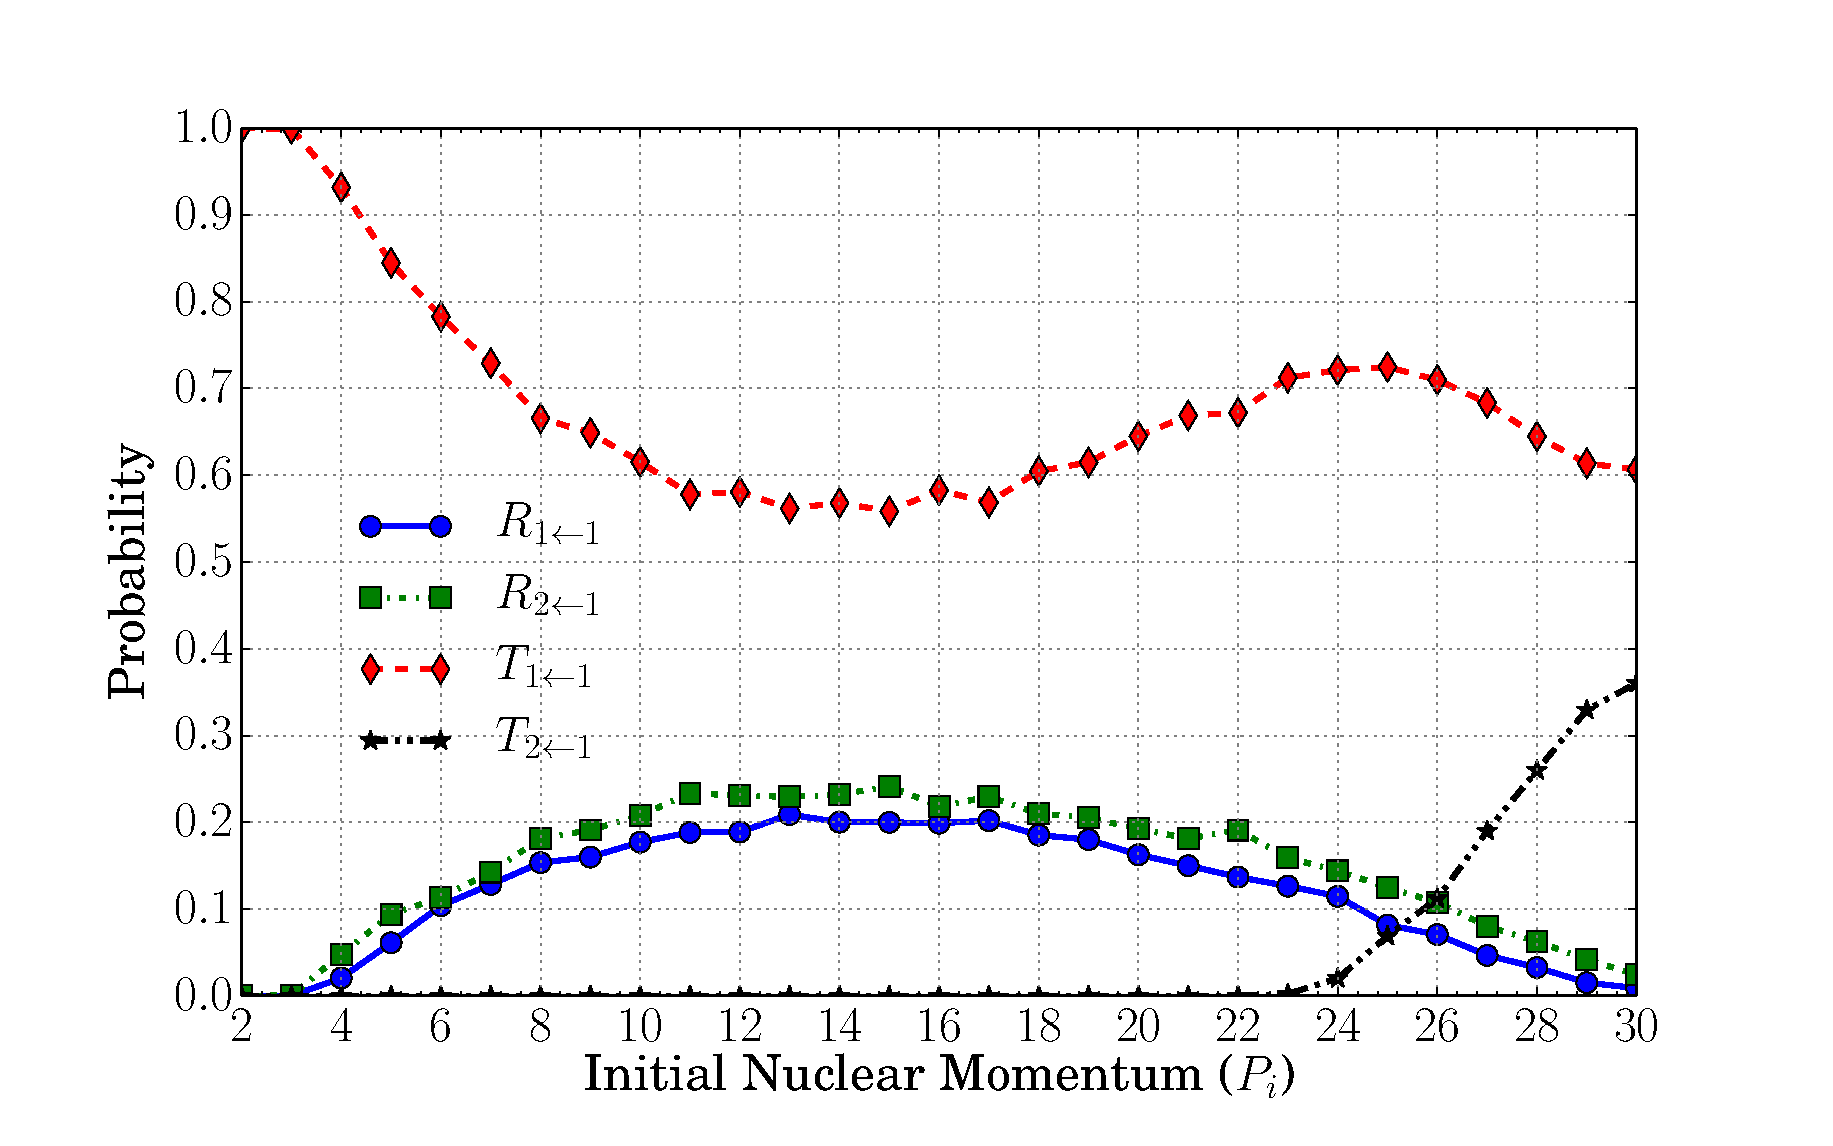
\includegraphics[scale=0.5]{ec_prob_1o5ip.eps}
\caption[Extended coupling: small integration step. $ i = 1 $.]{Transition probabilities for $ R $ and $ T $ for $ h = (5 P_{i})^{-1} $. $ i = 1 $.}
\label{f:ec1}
\end{figure}
\begin{figure}
\centering
\includegraphics[scale=0.5]{ec_prob_lh_mean.eps}
\caption[Extended coupling: large integration step. $ i = 1 $.]{Transition probabilities for $ R $ and $ T $ for $ (h = 0.10125 P_{i})^{-1}$. Mean of two 15,000 MC step runs, total of 30,000 MC steps. $ i = 1 $. Computational time $ = 48 + 49$ min. $ 55.44 + 26.91 $ s.}
\label{f:eclhmean}
\end{figure}
\Cref{f:ecpar} shows results from two parallel runs, they do not differ significantly from those of single-core calculations.
\begin{figure}
\centering
\includegraphics[scale=0.5]{ec_prob_parallel.eps}
\caption[Extended coupling: parallel calculations. $ i = 1 $.]{Parallel calculations on four cores (3750 per core) and $ h = (5 P_{i})^{-1} $. $ i = 1 $.}
\label{f:ecpar}
\end{figure}

Following the precedent, we shall start the analysis with $ i = 1 $. The behaviour of \too~at low momenta is due to the fact that $ E_{1} $ is highly attractive (see \cref{f:apesec}), so the particle is easily transmitted without strongly interacting with any other PES, as seen in \cref{sf:ect11,sf:ect11e}. However, as the momentum increases the particle starts interacting more strongly with the off-diagonal diabatic PES, and it becomes more likely to be reflected by it, with or without an electronic transition---as is observed in \cref{sf:ecr11,sf:ecr21}, giving rise to the bump in probability of \roo~and \rto, and the dip in the probability of \too. It is only at higher nuclear momenta that it is possible for the particle to experience an electronic transition and have enough momentum to work against the repulsive nature of $ E_{2} $---which is clearly seen in the sharp momentum drop in \cref{sf:ecr21}, which comes about by the switch in electronic state more closely observed in \cref{sf:ect21e}---leading to increased likelihood of observing \tto~transitions.

\begin{figure}
\vspace{-5mm}
\begin{subfigure}[t]{0.5\textwidth}
\centering
\includegraphics[width=\textwidth]{ec_traj_r11.eps}
\caption[Extended coupling: \roo~trajectory.]{\roo~trajectory.}
\label{sf:ecr11}
\end{subfigure}
~
\begin{subfigure}[t]{0.5\textwidth}
\centering
\includegraphics[width=\textwidth]{ec_traj_r11_e.eps}
\caption[Extended coupling: \roo~trajectory, zoom into $ n_{1}~\text{and}~n_{2} $.]{\roo~trajectory, zoom into $ n_{1}~\text{and}~n_{2} $.}
\label{sf:ecr11e}
\end{subfigure}
\\[-1mm]
\begin{subfigure}[t]{0.5\textwidth}
\centering
\includegraphics[width=\textwidth]{ec_traj_r21.eps}
\caption[Extended coupling: \rto~trajectory.]{\rto~trajectory.}
\label{sf:ecr21}
\end{subfigure}
~
\begin{subfigure}[t]{0.5\textwidth}
\centering
\includegraphics[width=\textwidth]{ec_traj_r21_e.eps}
\caption[Extended coupling: \rto~trajectory, zoom into $ n_{1}~\text{and}~n_{2} $.]{\rto~trajectory, zoom into $ n_{1}~\text{and}~n_{2} $.}
\label{sf:ecr21e}
\end{subfigure}
\\[-1mm]
\begin{subfigure}[t]{0.5\textwidth}
\centering
\includegraphics[width=\textwidth]{ec_traj_t11.eps}
\caption[Extended coupling: \too~trajectory.]{\too~trajectory.}
\label{sf:ect11}
\end{subfigure}
~
\begin{subfigure}[t]{0.5\textwidth}
\centering
\includegraphics[width=\textwidth]{ec_traj_t11_e.eps}
\caption[Extended coupling: \too~trajectory, zoom into $ n_{1}~\text{and}~n_{2} $.]{\too~trajectory, zoom into $ n_{1}~\text{and}~n_{2} $.}
\label{sf:ect11e}
\end{subfigure}
\\[-1mm]
\begin{subfigure}[t]{0.5\textwidth}
\centering
\includegraphics[width=\textwidth]{ec_traj_t21.eps}
\caption[Extended coupling: \tto~trajectory.]{\tto~trajectory.}
\label{sf:ect21}
\end{subfigure}
~
\begin{subfigure}[t]{0.5\textwidth}
\centering
\includegraphics[width=\textwidth]{ec_traj_t21_e.eps}
\caption[Extended coupling: \tto~trajectory, zoom into $ n_{1}~\text{and}~n_{2} $.]{\tto~trajectory, zoom into $ n_{1}~\text{and}~n_{2} $.}
\label{sf:ect21e}
\end{subfigure}
\vspace{-3mm}
\caption[Extended coupling: trajectory examples. $ i = 1 $.]{Trajectory examples. $ i = 1 $.}
\label{f:ec1t}
\end{figure}

\begin{figure}
\centering
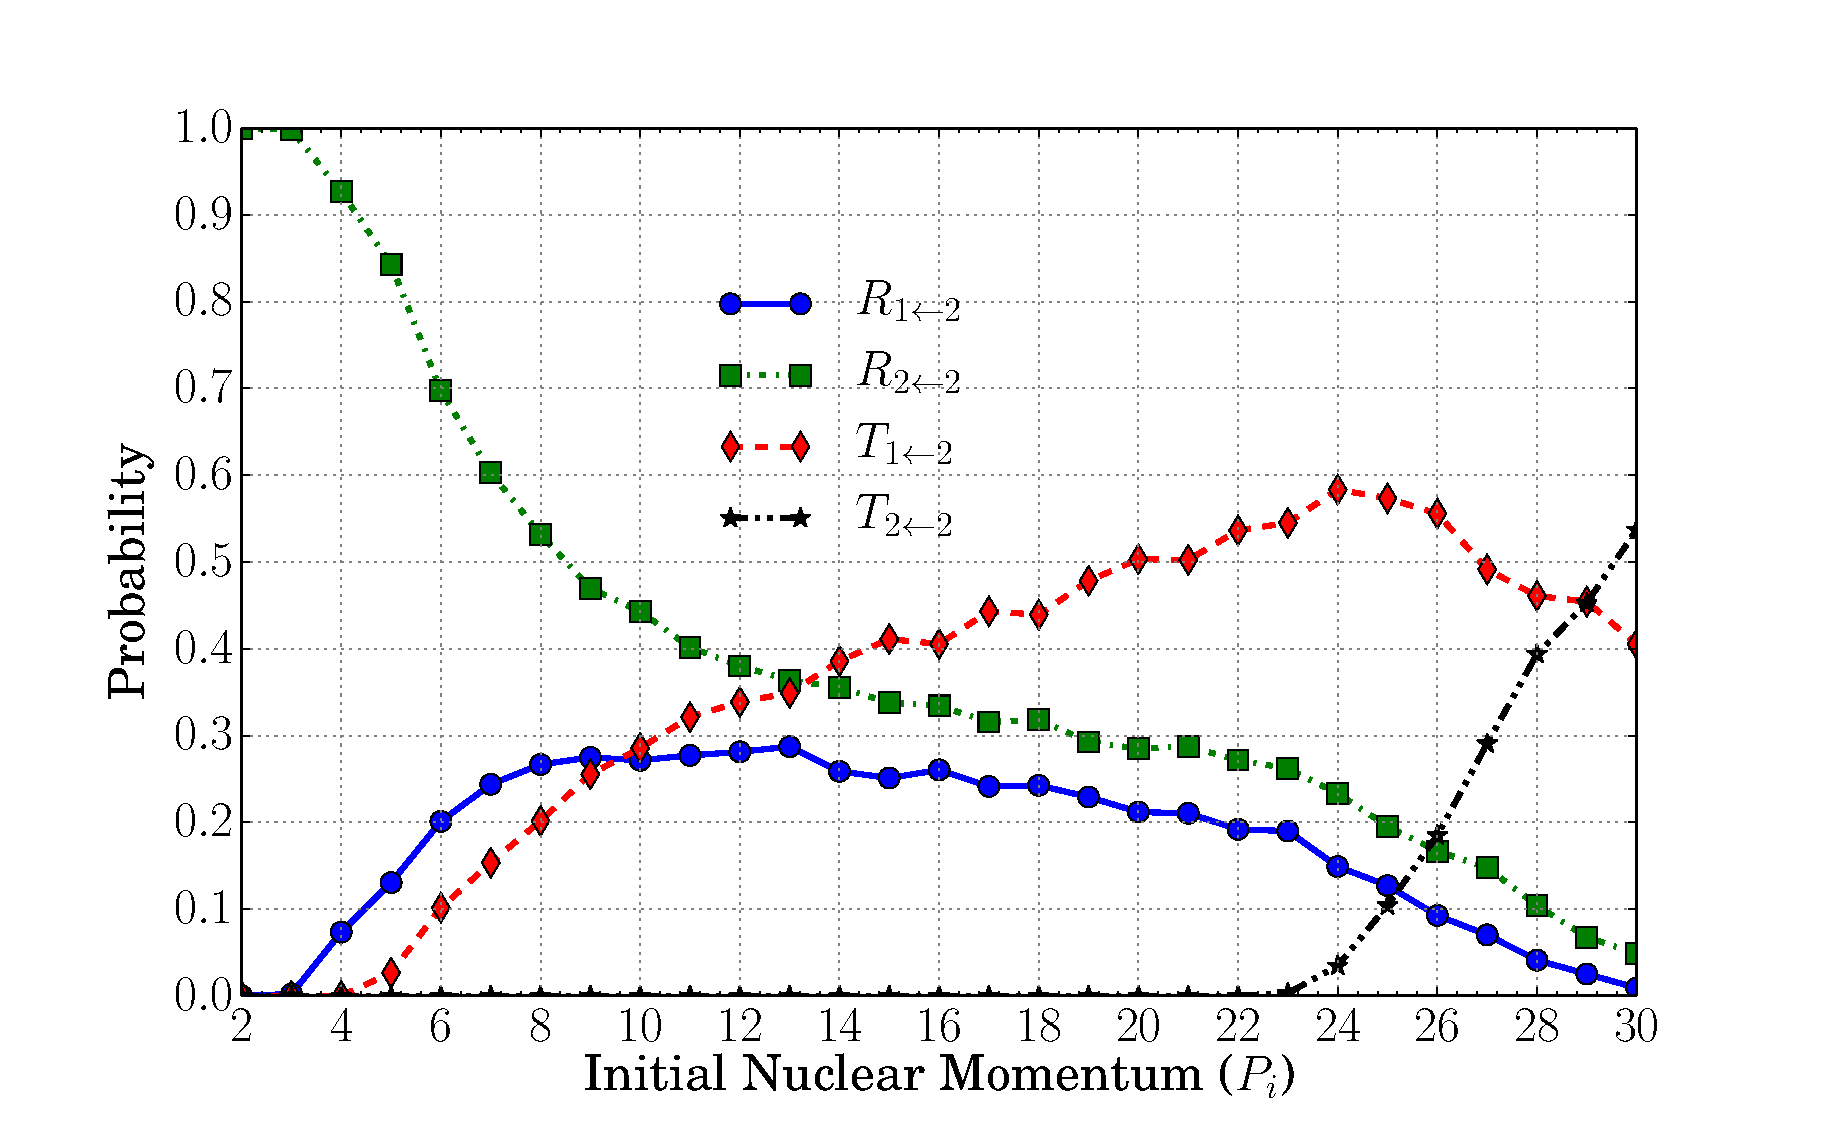
\includegraphics[scale=0.5]{ec_prob_i2.eps}
\caption[Extended coupling. $ i = 2 $]{Transition probabilities for $ R $ and $ T $ for $ h = (0.10125 P_{i})^{-1} $. $ i = 2 $. Computational time $ = 40$ min. $ 51.63 $ s.}
\label{f:ec2}
\end{figure}
When $ i = 2 $ as shown in \cref{f:ec2}, the system's behaviour changes drastically. At low nuclear momenta, the particle does not have the required energy to be transmitted or undergo an electronic transition---seen in \cref{sf:ecr22,sf:ecr22e}---and is simply reflected by the repulsive nature of $ E_{2} $, leading to the shape of \rtt. However, as nuclear momentum increases, the particle starts being able to change electronic state and be transmitted or reflected as observed in \cref{sf:ecr12,sf:ecr12e,sf:ect12,sf:ect12e}, leading to the increase in the probabilities of \rot~and \tot. As the momentum is increased further, the probability of having enough energy to transition into the lower electronic state and be transmitted increases, leading to the drop in \rtt~and \rot, and increase of \tot. As the nuclear momentum increases further, then the particle is travelling fast enough that it can overcome the repulsive effect of $ E_{2} $---as observed in \cref{sf:ect22,sf:ect22e}---and so it interacts relatively little with $ E_{1} $, leading to the increased probability of observing \ttt~transitions.

\begin{figure}
\vspace{-5mm}
\begin{subfigure}[t]{0.5\textwidth}
\centering
\includegraphics[width=\textwidth]{ec_traj_r12.eps}
\caption[Extended coupling: \rot~trajectory.]{\rot~trajectory.}
\label{sf:ecr12}
\end{subfigure}
~
\begin{subfigure}[t]{0.5\textwidth}
\centering
\includegraphics[width=\textwidth]{ec_traj_r12_e.eps}
\caption[Extended coupling: \rot~trajectory, zoom into $ n_{1}~\text{and}~n_{2} $.]{\rot~trajectory, zoom into $ n_{1}~\text{and}~n_{2} $.}
\label{sf:ecr12e}
\end{subfigure}
\\[-1mm]
\begin{subfigure}[t]{0.5\textwidth}
\centering
\includegraphics[width=\textwidth]{ec_traj_r22.eps}
\caption[Extended coupling: \rtt~trajectory.]{\rtt~trajectory.}
\label{sf:ecr22}
\end{subfigure}
~
\begin{subfigure}[t]{0.5\textwidth}
\centering
\includegraphics[width=\textwidth]{ec_traj_r22_e.eps}
\caption[Extended coupling: \rtt~trajectory, zoom into $ n_{1}~\text{and}~n_{2} $.]{\rtt~trajectory, zoom into $ n_{1}~\text{and}~n_{2} $.}
\label{sf:ecr22e}
\end{subfigure}
\\[-1mm]
\begin{subfigure}[t]{0.5\textwidth}
\centering
\includegraphics[width=\textwidth]{ec_traj_t12.eps}
\caption[Extended coupling: \tot~trajectory.]{\tot~trajectory.}
\label{sf:ect12}
\end{subfigure}
~
\begin{subfigure}[t]{0.5\textwidth}
\centering
\includegraphics[width=\textwidth]{ec_traj_t12_e.eps}
\caption[Extended coupling: \tot~trajectory, zoom into $ n_{1}~\text{and}~n_{2} $.]{\tot~trajectory, zoom into $ n_{1}~\text{and}~n_{2} $.}
\label{sf:ect12e}
\end{subfigure}
\\[-1mm]
\begin{subfigure}[t]{0.5\textwidth}
\centering
\includegraphics[width=\textwidth]{ec_traj_t22.eps}
\caption[Extended coupling: \ttt~trajectory.]{\ttt~trajectory.}
\label{sf:ect22}
\end{subfigure}
~
\begin{subfigure}[t]{0.5\textwidth}
\centering
\includegraphics[width=\textwidth]{ec_traj_t22_e.eps}
\caption[Extended coupling: \ttt~trajectory, zoom into $ n_{1}~\text{and}~n_{2} $.]{\ttt~trajectory, zoom into $ n_{1}~\text{and}~n_{2} $.}
\label{sf:ect22e}
\end{subfigure}
\vspace{-3mm}
\caption[Extended coupling: trajectory examples. $ i = 2 $]{Trajectory examples. $ i = 2 $.}
\label{f:ec2t}
\end{figure}
%
\section{Spin-Boson Model for Condensed-Phase Dynamics}
%
Some details were left out of \cite{project} in regards to this problem---namely the value of $ \omega_{c} $, and the range and distribution of $ \omega_{k} $ (defined in \cref{sb:sb})---so it was assumed that $ \omega_{c} = 1$, and everything else was defined from there, which means there is no standard with which to compare results. \Cref{f:sb1,f:sb2} show the results of eight systems in total: two symmetric and two asymmetric for $ i = 1,2 $ each. The calculations were carried out for 100 nuclei ($ M=100 $).

\begin{figure}
\begin{subfigure}{\textwidth}
\centering
\includegraphics[width=\textwidth]{spin_boson_e11.eps}
\caption{$ i = 1 $. For both systems $ h = 0.01$. Computational time symmetric: $ 8 $ hrs. $ 46 $ min. $ 24.33 $ s.; asymmetric: $ 3 $ hrs. $ 32 $ min. $ 37.54 $ s.}
\label{f:sbe11}
\end{subfigure}

\begin{subfigure}{\textwidth}
\centering
\includegraphics[width=\textwidth]{spin_boson_e12.eps}
\caption{$ i = 2 $. For the symmetric problem, $ h = 0.1 $ and MC reps $ = 5000 $. For the asymmetric problem, $ h = 0.01 $ and MC reps $ = 30000 $. Computational time symmetric: $ 1 $ hrs. $ 16 $ min. $ 0.12 $ s.; asymmetric: $ 3 $ hrs. $ 44 $ min. $ 9.44 $ s.}
\label{f:sbe12}
\end{subfigure}
\caption{Spin-boson calculations for symmetric ($ \epsilon = 0 $) and asymmetric ($ \epsilon = 1 $) systems. $\alpha = 0.09,~\beta = 0.25,~\Delta = (2.5)^{-1}$.}
\label{f:sb1}
\end{figure}
\Cref{f:sb1} shows incoherent (non-oscillatory) relaxation dynamics for all four systems. It is particularly interesting how much the behaviour changes between the symmetric and asymmetric version of each problem. In both cases, the asymmetric system favours the second state. Which means that the second state has a lower energy than the first. This notion is also evidenced by the fact that both symmetric systems also stabilise at negative values of $ D(t) $, signifying that the probability of finding the system in state 2 is higher than that of finding it in state 1. This can potentially be observed from \cref{eq:sbpes1,eq:sbpes2}.

\begin{figure}
\begin{subfigure}{\textwidth}
\centering
\includegraphics[width=\textwidth]{spin_boson_e21.eps}
\caption{$ i = 1 $. For the symmetric problem, $ h = 0.1 $ and MC reps $ = 5000 $. For the asymmetric problem, $ h = 0.05 $ and MC reps $ = 30000 $. Computational time symmetric: $ 1 $ hrs. $ 43 $ min. $ 32.96 $ s.; asymmetric: $ 16 $ hrs. $ 58 $ min. $ 5.03 $ s.}
\label{f:sbe21}
\end{subfigure}

\begin{subfigure}{\textwidth}
\centering
\includegraphics[width=\textwidth]{spin_boson_e22.eps}
\caption{$ i = 2 $. For the symmetric problem, $ h = 0.1 $ and MC reps $ = 5000 $. For the asymmetric problem, $ h = 0.05 $ and MC reps $ = 30000 $. Computational time symmetric: $ 1 $ hrs. $ 52 $ min. $ 0.86 $ s.; asymmetric: $ 46 $ min. $ 17.54 $ s.}
\label{f:sbe22}
\end{subfigure}
\caption{Spin-boson calculations for symmetric ($ \epsilon = 0 $) and asymmetric ($ \epsilon = 1 $) systems. $\alpha = 0.1,~\beta = 12.5,~\Delta = (2.5)^{-1}$.}
\label{f:sb2}
\end{figure}
On the other hand, \cref{f:sb2} shows both, coherent (oscillatory) and non-coherent (non-oscillatory) relaxation dynamics. For both initial states, the symmetric system manifests highly oscillatory behaviour. But the surprising results arise from their asymmetric counterparts. This means that for our chosen parameters, the dynamical system described by the equations of motion has large regions of stability in the electronic phase space. Such phenomena are not unheard of---where the same equations with different parameters yield vastly different results, ranging from nicely behaved to chaotic systems. Suffice to say, this was completely unexpected (and probably highly coincidental).

To conclude with this discussion, it must be said that the disparity in integration step and MC reps is down to each individual system's run time. The aforementioned quantities were adjusted so that no run exceeded 17 hours. There was some overcompensation in a few systems due to the highly variable nature of their run times, which in one instance was observed to exceed $ 250000\% $, though less extreme examples fell in the range of $ 300\%~\text{to}~1000\% $. This phenomenon is attributed to the large number of uniformly and normally distributed random numbers required to set the initial conditions, as some of them do not allow the selection criteria to be met. The problem was compounded by the random seed allocation at every MC rep, and by the fact that the selection criteria (\cref{eq:select}) must be met at every plot point, otherwise the MC rep has to be restarted.
%
\section{Parallelisation and Scaling}
%
\begin{figure}[!htbp]
\centering
\includegraphics[width=0.7\textwidth]{mpi.eps}
\caption[Time scaling as a function of the number of cores and Monte-Carlo repetitions.]{Time scaling as a function of the number of cores and MC reps. After 4 cores, Open MPI starts utilising the processor's hyper-threading capabilities. \texttt{mpirun} runs copies of the program on the number of specified cores, meaning that the slower copies progressively overwrite the faster ones' files, thus making the slowest execution time the only surviving measurement. This means that $ t \propto n^{-1}$, where $ t \equiv $ time and $ n \equiv $ \# of cores used. It also shows that $ t $ scales linearly with the number of MC reps. Test system: single avoided crossing.}
\end{figure}